
\section{Tensors}


\begin{frame}
  \frametitle{What is a Tensor?}

  Tensors are used to described linear interactions between physical
  properties.

  \pause

  \begin{description}
    \item[rank zero tensor] scalar property, e.g. temperature
    \item[rank one tensor] directional depended property, e.g. wave velocity
    \item[rank two tensors] relationship between two vector fields,
    e.g. stress, strain, conductivity
    \item[rank three tensor] relationship between a one and a two rank tensor,
    e.g. piezoelectricity
    \item[rank four tensor] relationship between two two rank tensor, e.g. elasticity,
  \end{description}

  \pause

  A tensor $T$ of rank $s+t$ maps a tensor $A$ of rank $s$ onto a tensor $B$
  of rank $t$ by the formula
  \begin{equation*}
    B_{k_{1},\ldots,k_{t}}
    = T_{k_{1},k_{2},\ldots,k_{t},j_{1},\ldots,j_{s}} A_{j_{1},\ldots,j_{s}}
  \end{equation*}

\end{frame}


\begin{frame}[fragile]
  \frametitle{A Simple Example}


  \begin{lstlisting}
M = [[1.45 0.00 0.19];...
     [0.00 2.11 0.00];...
     [0.19 0.00 1.79]];

sigma = tensor(M,'name','stress','unit','MPa');
\end{lstlisting}
\begin{onlyenv}<1>
  \begin{lstlisting}[style=output]
sigma = stress tensor (show methods, plot)
  unit: MPa
  rank: 2 (3 x 3)

  1.45 0 0.19
  0 2.11 0
  0.19 0 1.79
  \end{lstlisting}
\end{onlyenv}

\pause
\medskip

\begin{lstlisting}
n = vector3d(1,0,0) % normal direction
\end{lstlisting}
\begin{onlyenv}<2>
  \begin{lstlisting}[style=output]
n = vector3d (show methods, plot)
  size: 1 x 1
  x y z
  1 0 0
  \end{lstlisting}
\end{onlyenv}

\pause
\medskip

the stress vector $T^{\vec n}$ of plane $\vec n = \{1,0,0\}$, is computed by
$T^{\vec n}_{j} = \sigma_{ij} \vec n_{i}.$

\pause
\medskip

\begin{lstlisting}
T = EinsteinSum(sigma,[-1 1],n,-1,'unit','MPa')
\end{lstlisting}
\begin{lstlisting}[style=output]
T = tensor (show methods, plot)
  unit: MPa
  rank: 1 (3)

 1.45
    0
 0.19
\end{lstlisting}


\end{frame}



\begin{frame}[fragile]
  \frametitle{Einstein Summation}

  The scalar magnitudes of the normal stress $\sigma_{N}$ and the shear stress
  $\sigma_{S}$ are given as
  \begin{equation*}
    \sigma_{N} = T^{\vec n}_{i} \vec n_{i} = \sigma_{ij} \vec n_{i}\vec n_{j}
    \quad \text{ and } \quad
    \sigma_{S} =\sqrt{T^{\vec n}_{i}T^{\vec n}_{i} - \sigma^{2}_{N} }.
  \end{equation*}

  \medskip
  \pause

\begin{lstlisting}
sigmaN = double(EinsteinSum(T,-1,n,-1))
sigmaS = sqrt(double(EinsteinSum(T,-1,T,-1))...
         - sigmaN^2)
\end{lstlisting}
\begin{lstlisting}[style=output]
sigmaN =

    1.4500

sigmaS =

    0.1900
\end{lstlisting}

\end{frame}



\begin{frame}[fragile]
  \frametitle{Field Tensors vs. Matter Tensors}

  \begin{description}
    \item[field tensors] applied forces, like stress, strain,
  or a electric field
  \item[matter tensors] physical properties like electrical or thermal conductivity,
  magnetic permeability, etc., of a crystalline specimen
  \end{description}

\pause
\medskip

\begin{lstlisting}
S = symmetry('triclinic','mineral','Talc');
\end{lstlisting}

\pause
\medskip

\begin{onlyenv}<3>
  \begin{lstlisting}
M = [[219.8  59.6  -4.8 -0.8 -33.8 -1.0];...
     [ 59.6 216.3  -3.6  1.7 -16.5 -0.6];...
     [ -4.8  -3.6  48.8  4.1 -15.5 -3.5];...
     [ -0.8   1.7   4.1 26.5  -3.6 -6.4];...
     [-33.8 -16.5 -15.5 -3.6  22.8 -1.6];...
     [ -1.0  -0.6  -3.5 -6.4  -1.6 78.2]];

C = tensor(M,'name','stiffness','unit','GPa',S)
  \end{lstlisting}
\end{onlyenv}
\begin{onlyenv}<4->
\begin{lstlisting}
C = tensor(M,'name','stiffness','unit','GPa',S)
\end{lstlisting}
\end{onlyenv}

\pause

\begin{onlyenv}<4>
\begin{lstlisting}[style=output]
C = elastic stiffness tensor (size: 3 3 3 3)
     unit: GPa
     rank: 4
  mineral: Talc (triclinic, X||a*, Z||c)

  tensor in Voigt matrix representation
  219.83    59.66   -4.82  -0.82  -33.87   -1.04
   59.66   216.38   -3.67   1.79  -16.51   -0.62
   -4.82    -3.67   48.89   4.12  -15.52   -3.59
   -0.82     1.79    4.12  26.54   -3.60   -6.41
  -33.87   -16.51  -15.52  -3.60   22.85   -1.67
   -1.04    -0.62   -3.59  -6.41   -1.67   78.29
\end{lstlisting}
\end{onlyenv}

\pause
\medskip

import a tensor from the \emph{Material Properties Open Database}

\begin{lstlisting}
T = loadTensor('1000055.mpod')
\end{lstlisting}

\end{frame}


\begin{frame}[fragile]
  \frametitle{Visualization}

  \begin{columns}
    \begin{column}{8.3cm}

      For a second order tensor $k_{ij}$ its magnitude $R(\vec x)$ is defined as
      \begin{equation*}
        R(\vec x) = k_{ij} \vec x_{i} \vec x_{j}.
      \end{equation*}

\pause
\medskip

\begin{lstlisting}
x = Miller(1,0,0,S,'uvw');

R = EinsteinSum(k,[-1 -2],x,-1,x,-2)
\end{lstlisting}

\pause
\medskip


\begin{lstlisting}
R = directionalMagnitude(k,x)
\end{lstlisting}


\pause
\medskip

  \begin{lstlisting}
plot(k)
colorbar
  \end{lstlisting}

    \end{column}
    \begin{column}{4cm}
      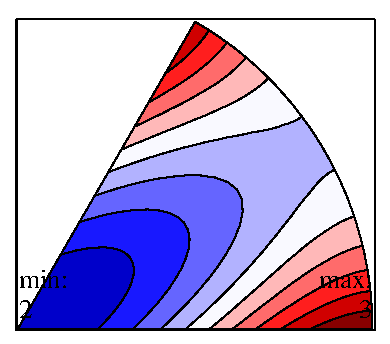
\includegraphics[width=4cm]{pic/tensor1}

      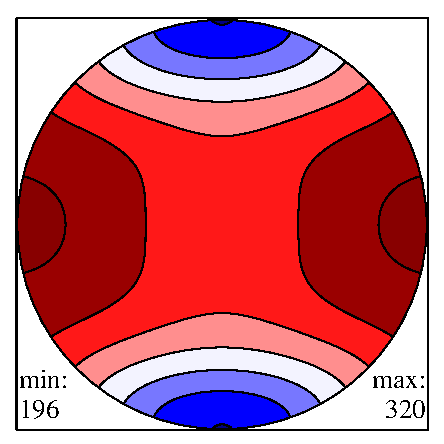
\includegraphics[width=4cm]{pic/tensor}
    \end{column}

  \end{columns}

\end{frame}



\begin{frame}[fragile]
  \frametitle{Rotating Tensors}

  the orientation of a certain crystal
  \begin{lstlisting}
R = orientation('Euler',10*degree,20*degree,0,S)
  \end{lstlisting}

\medskip
\pause

the elastic stiffness tensor in specimen coordinates
\begin{lstlisting}
C_rotated = rotate(C,g)
\end{lstlisting}
\begin{lstlisting}[style=output]
C_rotated = stiffness tensor
  unit: GPa
  rank: 4

  tensor in Voigt matrix representation
  228.7  56.0   1.9 19.9 -13.8  6.8
   56.0 176.0  11.6 50.3  -7.6  4.4
    1.9  11.6  43.2  5.2 -19.4  2.3
   19.9  50.3   5.2 43.4  -1.7  0.2
  -13.8  -7.6 -19.4 -1.7  29.3 17.3
    6.8   4.4   2.3  0.2  17.3  73.
\end{lstlisting}



\end{frame}





\begin{frame}[fragile,fragile,fragile]
  \frametitle{Average Tensors}

The average tensorial property of a specimen can be computed as the average of
the rotated matter tensors of each grain.

\medskip
\pause

The Voigt and the Reuss averages of a tensor $T$ are defines as
\begin{equation*}
  \left<T\right>^{\text{Voigt}}
  = \sum_{m=1}^{M} V_{m} T(g_{m}^{c}), \quad
  \left<T\right>^{\text{Reuss}}
  = \left[ \sum_{m=1}^{M} V_{m} T^{-1}(g_{m}^{c}) \right]^{-1}.
\end{equation*}

\medskip
\pause

For EBSD data this is computed by
\begin{lstlisting}
Tmean = calcTensor(ebsd,T,'Voigt')
\end{lstlisting}

\medskip
\pause

and for an ODF by
\begin{lstlisting}
Tmean = calcTensor(odf,T,'Voigt')
\end{lstlisting}



\end{frame}

\begin{frame}[fragile]
  \frametitle{Elasticity Tensors}

elastic compliance $S$ vs. elastic stiffness $C$
  \begin{lstlisting}
S = inv(C)
  \end{lstlisting}

  \begin{onlyenv}<1>
\begin{lstlisting}[style=output]
S = compliance tensor (show methods, plot)
  unit   : 1/GPa
  rank   : 4 (3 x 3 x 3 x 3)
  mineral: Talc (triclinic, X||a*, Z||c)

  tensor in Voigt matrix representation: *10^-3
  6.9 -0.8  4.7  0.7  6.5  0.3
 -0.8  5.1  1.4 -0.0  1.7  0.0
  4.7  1.4 30.3 -0.1 14.3  0.9
   0. -0.0 -0.1  9.9  2.1  0.8
  6.5  1.7 14.3  2.1 21.7  0.9
  0.3  0.0  0.9  0.8  0.9  3.3
\end{lstlisting}
\end{onlyenv}

\pause
\medskip

stress $\sigma$ vs. strain $\varepsilon$
  \begin{lstlisting}
epsilon = EinsteinSum(S,[-1 -2 1 2],sigma,[-1 -2])
  \end{lstlisting}

  \begin{onlyenv}<2>
\begin{lstlisting}[style=output]
S = strain tensor (show methods, plot)
  rank   : 2 (3 x 3)
  mineral: Talc (triclinic, X||a*, Z||c)

    423   -9.6 -102.9
   -9.6  530.1    8.4
 -102.9    8.4   66.9
\end{lstlisting}
\end{onlyenv}

\pause
\medskip

\begin{onlyenv}<3->

  \begin{columns}
    \begin{column}{7.7cm}

      derived elastic properties
\begin{lstlisting}
beta = volumeCompressibility(C)
beta = linearCompressibility(C,x)
E    = YoungsModulus(C,x)
G    = shearModulus(C,h,u)
nu   = PoissonRatio(C,x,y)
T    = ChristoffelTensor(C,n)
\end{lstlisting}


\begin{lstlisting}
plot(C,'PlotType',YoungsModulus')
\end{lstlisting}

    \end{column}
    \begin{column}{4cm}
      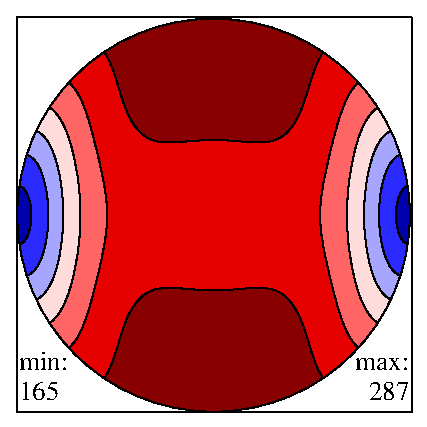
\includegraphics[width=4cm]{pic/YM}
    \end{column}
  \end{columns}
\end{onlyenv}
\end{frame}


\begin{frame}[fragile]
  \frametitle{Wave Velocities}

\begin{lstlisting}
[vp,vs1,vs2,pp,ps1,ps2] = velocity(C,xvector,rho)
\end{lstlisting}

  \begin{columns}
  \begin{column}{8.5cm}

\begin{lstlisting}
plot(C,'PlotType','velocity','vp')

hold on
plot(C,'PlotType','velocity','pp')
hold off
\end{lstlisting}

\bigskip
\pause

    \begin{lstlisting}
plot(C,'PlotType','velocity','vs1-vs2')

hold on
plot(C,'PlotType','velocity','ps1')
hold off
\end{lstlisting}

  \end{column}
    \begin{column}{3.5cm}
      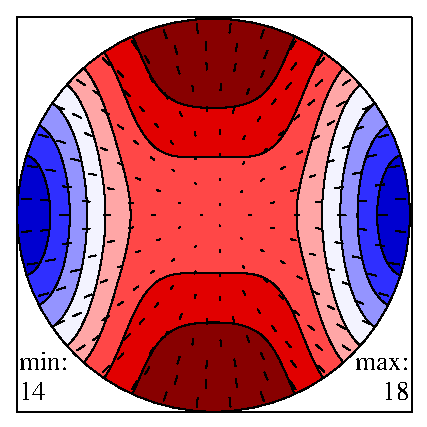
\includegraphics[width=3.5cm]{pic/vp-pp}

      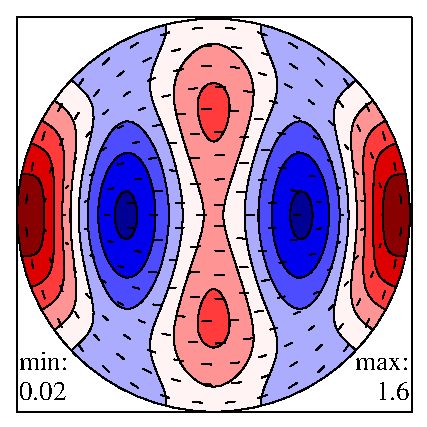
\includegraphics[width=3.5cm]{pic/vs12-ps1}
  \end{column}

  \end{columns}

\end{frame}

\subsection*{Exercises}

\begin{frame}

  \begin{Exercise}
    \begin{enumerate}[a)]
      \item Load the EBSD data:
      \texttt{data/ebsd/85\_829grad\_07\_09\_06.txt}.
      \item Estimate an ODF from the above EBSD data.
      \item Visualize the ODF and some of its pole figures.
      \item Explore the influence of the halfwidth on the kernel
      density estimation by looking at the pole figures! Which kernel is the best?
      \item Compute the optimal kernel by the command \texttt{calcKernel}.
    \end{enumerate}
  \end{Exercise}

    \begin{Exercise}
      Do the same as above with a model ODF, i.e.
    \begin{enumerate}[a)]
      \item define a model ODF
      \item simulate EBSD from this ODF
      \item estimate the ODF back from these EBSD data
      \item compare the estimated ODF with the original ODF
      \item explore the influence of the halfwidth of the kernel function
    \end{enumerate}
  \end{Exercise}

\end{frame}

%%% Local Variables:
%%% mode: latex
%%% TeX-master: "main"
%%% End:
